\documentclass[11pt,letterpaper]{article}
\usepackage[margin=1in]{geometry}
\usepackage[T1]{fontenc}
\usepackage[utf8]{inputenc}
\usepackage{lmodern}
\usepackage{microtype}
\usepackage{graphicx}
\usepackage{booktabs}
\usepackage{float}
\usepackage{hyperref}
\usepackage{caption}
\usepackage{setspace}
\setstretch{1.15}
\setlength{\parindent}{0pt}
\setlength{\parskip}{0.65em}
\hypersetup{colorlinks=true,urlcolor=blue,linkcolor=black}
\title{Exploring Gene Expression Patterns in Breast Cancer\\Using TCGA-BRCA RNA-seq Data}
\author{Arwa Gulzar}
\date{October 2026}
\begin{document}
\maketitle
\section{Introduction}
Breast cancer is a biologically diverse disease characterized by differences in gene expression, tumor behavior, and response to treatment. Understanding these differences is important for identifying molecular characteristics that distinguish breast cancer subtypes and influence clinical outcomes. Advances in RNA sequencing (RNA-seq) have made it possible to examine gene expression across large collections of tumor samples, providing valuable information about the molecular features of cancer.

This analysis utilizes RNA-seq gene count data and associated sample metadata from The Cancer Genome Atlas Breast Invasive Carcinoma (TCGA-BRCA) project. The dataset contains gene expression measurements across 1,231 samples, allowing for the investigation of variation in gene expression and its relationship to molecular breast cancer subtypes.

Two genes, \textit{ESR1} (estrogen receptor 1) and \textit{PGR} (progesterone receptor), were selected for analysis because of their biological relevance to hormone receptor signaling in breast cancer. \textit{ESR1} encodes estrogen receptor alpha, a protein involved in estrogen-dependent cellular signaling and the regulation of gene transcription. \textit{PGR} encodes the progesterone receptor, whose expression is associated with hormone receptor activity. Both genes are relevant to the molecular characterization of breast cancer and the distinction between hormone receptor-associated and other tumor subtypes.

The primary objective of this analysis was to characterize the distribution of \textit{ESR1} and \textit{PGR} RNA-seq counts, examine their relationship across samples, and investigate differences in \textit{ESR1} expression among PAM50 breast cancer subtypes. Summary statistics and multiple visualization techniques, including a histogram, scatter plot, box plot, heatmap, and density plot, were used to identify patterns and variation within the dataset.

\section{Methods}
RNA-seq gene count data and corresponding sample metadata from The Cancer Genome Atlas Breast Invasive Carcinoma (TCGA-BRCA) project were analyzed using R. The dataset contained expression measurements for 60,660 genes across 1,231 samples. The count matrix and metadata were imported as CSV files, and the sample identifiers were matched to ensure that gene expression measurements corresponded to the correct sample annotations.

Two genes, \textit{ESR1} (ENSG00000091831) and \textit{PGR} (ENSG00000082175), were selected based on their relevance to hormone receptor signaling in breast cancer. The mean, median, standard deviation, minimum, and maximum raw RNA-seq counts were calculated for each gene to summarize their distributions.

Five visualization techniques were used to examine gene expression patterns. A histogram displayed the distribution of \textit{ESR1} counts, while a scatter plot examined the relationship between \textit{ESR1} and \textit{PGR} counts across samples. A box plot compared \textit{ESR1} expression across PAM50 breast cancer subtypes, and a density plot further illustrated differences in the distributions of \textit{ESR1} counts among these subtypes. A heatmap displayed the 10 genes with the highest average raw counts, using hierarchical clustering to identify similarities in expression patterns across samples. PAM50 subtype annotations were included to provide additional biological context.

For visualization, raw counts were transformed using $\log_2(\mathrm{count}+1)$ to reduce the influence of extreme values and improve the visibility of expression patterns. Samples with missing PAM50 subtype information were excluded from the box plot and density plot. The analysis remained descriptive, and no inferential statistical tests were performed.

Data manipulation and visualization were performed using the tidyverse (version 2.0.0), including ggplot2 (version 4.0.3). ComplexHeatmap (version 2.28.0) was used to construct the heatmap, and circlize (version 0.4.18) was loaded to support its visualization framework. Summary statistics were calculated using base R functions, and the results were organized and displayed using knitr.

\section{Results}
\subsection{Summary Statistics}
Descriptive statistics were calculated for \textit{ESR1} and \textit{PGR} across 1,231 TCGA-BRCA samples (Table 1). \textit{ESR1} had a mean raw count of 31,442.22 and a median of 17,561, while \textit{PGR} had a mean of 8,791.82 and a median of 2,382. The standard deviations were 38,261.25 for \textit{ESR1} and 17,529.30 for \textit{PGR}, indicating substantial variation across samples. Both genes had means greater than their medians, consistent with right-skewed raw count distributions.

\begin{table}[H]
\centering
\caption{Summary statistics for ESR1 and PGR raw RNA-seq counts}
\label{tab:stats}
\small
\begin{tabular}{lrrrrr}
\toprule
Gene & Mean & Median & Standard Deviation & Minimum & Maximum \\
\midrule
\textit{ESR1} & 31,442.22 & 17,561 & 38,261.25 & 14 & 270,977 \\
\textit{PGR} & 8,791.82 & 2,382 & 17,529.30 & 1 & 345,065 \\
\bottomrule
\end{tabular}
\end{table}
\subsection{Histogram of \textit{ESR1} Expression}
The histogram of log2-transformed \textit{ESR1} counts (Figure 1) showed substantial variation across breast cancer samples. Most observations were concentrated around log2 expression values of 14--16, while another group of samples exhibited lower expression values. The $\log_2(\mathrm{count}+1)$ transformation reduced the influence of extremely high raw counts, allowing the distribution to be visualized more clearly.

\begin{figure}[H]
\centering
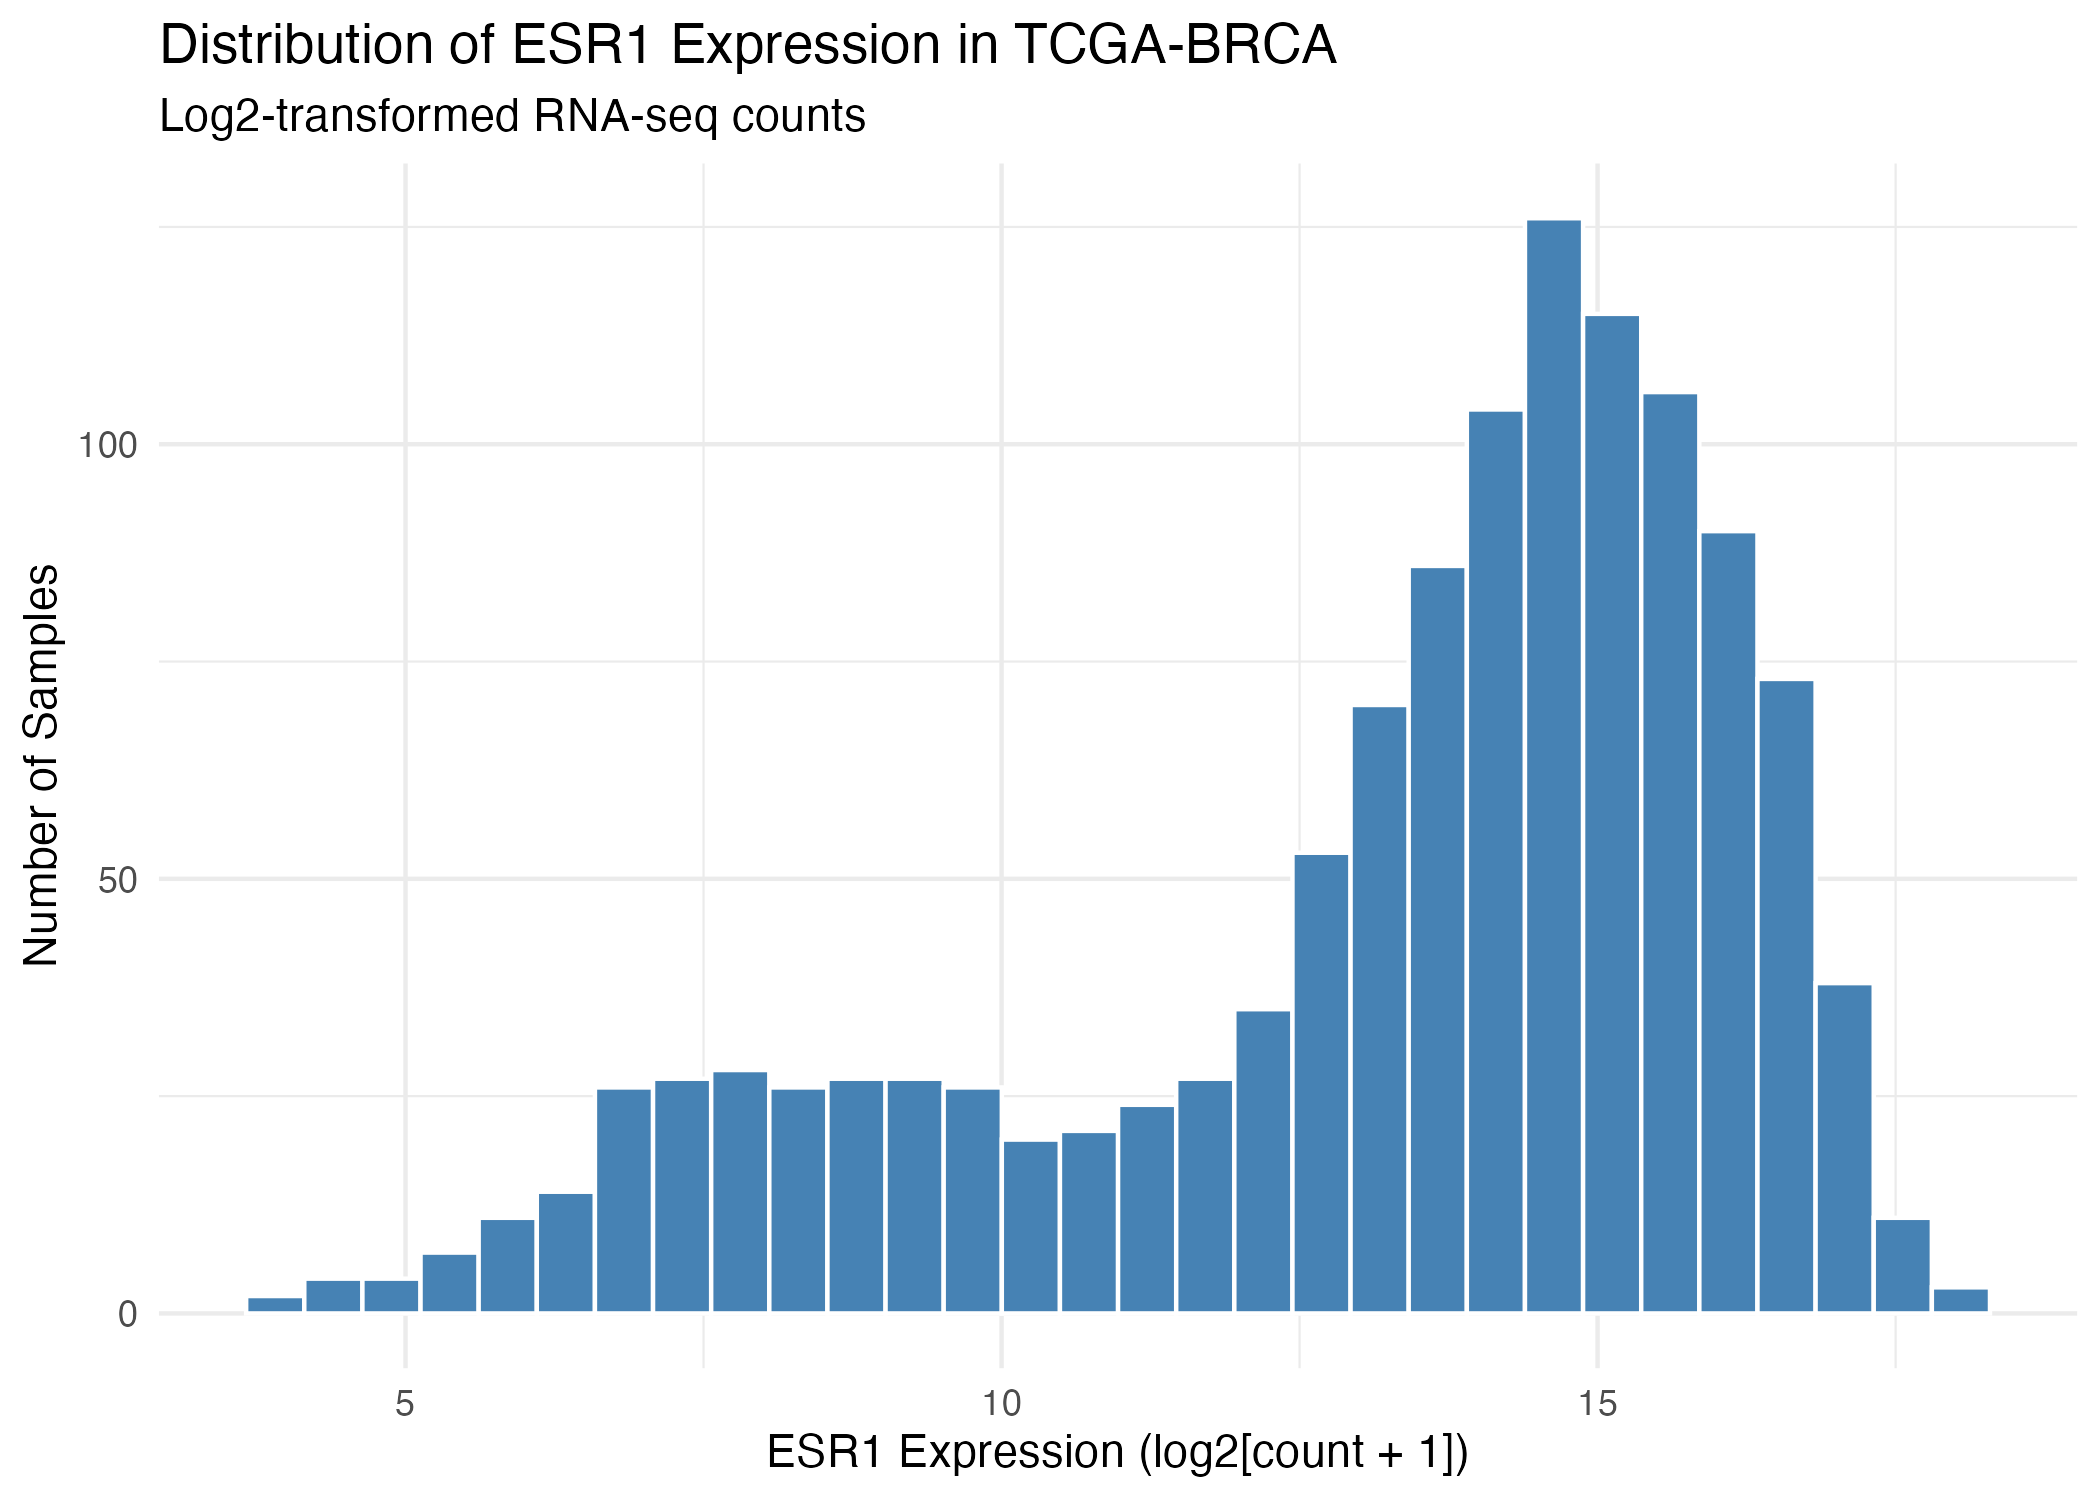
\includegraphics[width=\linewidth,height=0.52\textheight,keepaspectratio]{figures/histogram.png}
\caption{Distribution of log2-transformed \textit{ESR1} RNA-seq counts across TCGA-BRCA samples.}
\label{fig:histogram}
\end{figure}
\subsection{Relationship Between \textit{ESR1} and \textit{PGR} Expression}
The scatter plot comparing log2-transformed \textit{ESR1} and \textit{PGR} counts (Figure 2) suggested a general positive association between the two genes. Samples with higher \textit{ESR1} counts often exhibited higher \textit{PGR} counts, although considerable variation was observed. The relationship was not perfectly linear, indicating that samples with similar \textit{ESR1} expression could have different levels of \textit{PGR} expression. Transparency was applied to the plotted points to improve the visibility of overlapping observations.

\begin{figure}[H]
\centering
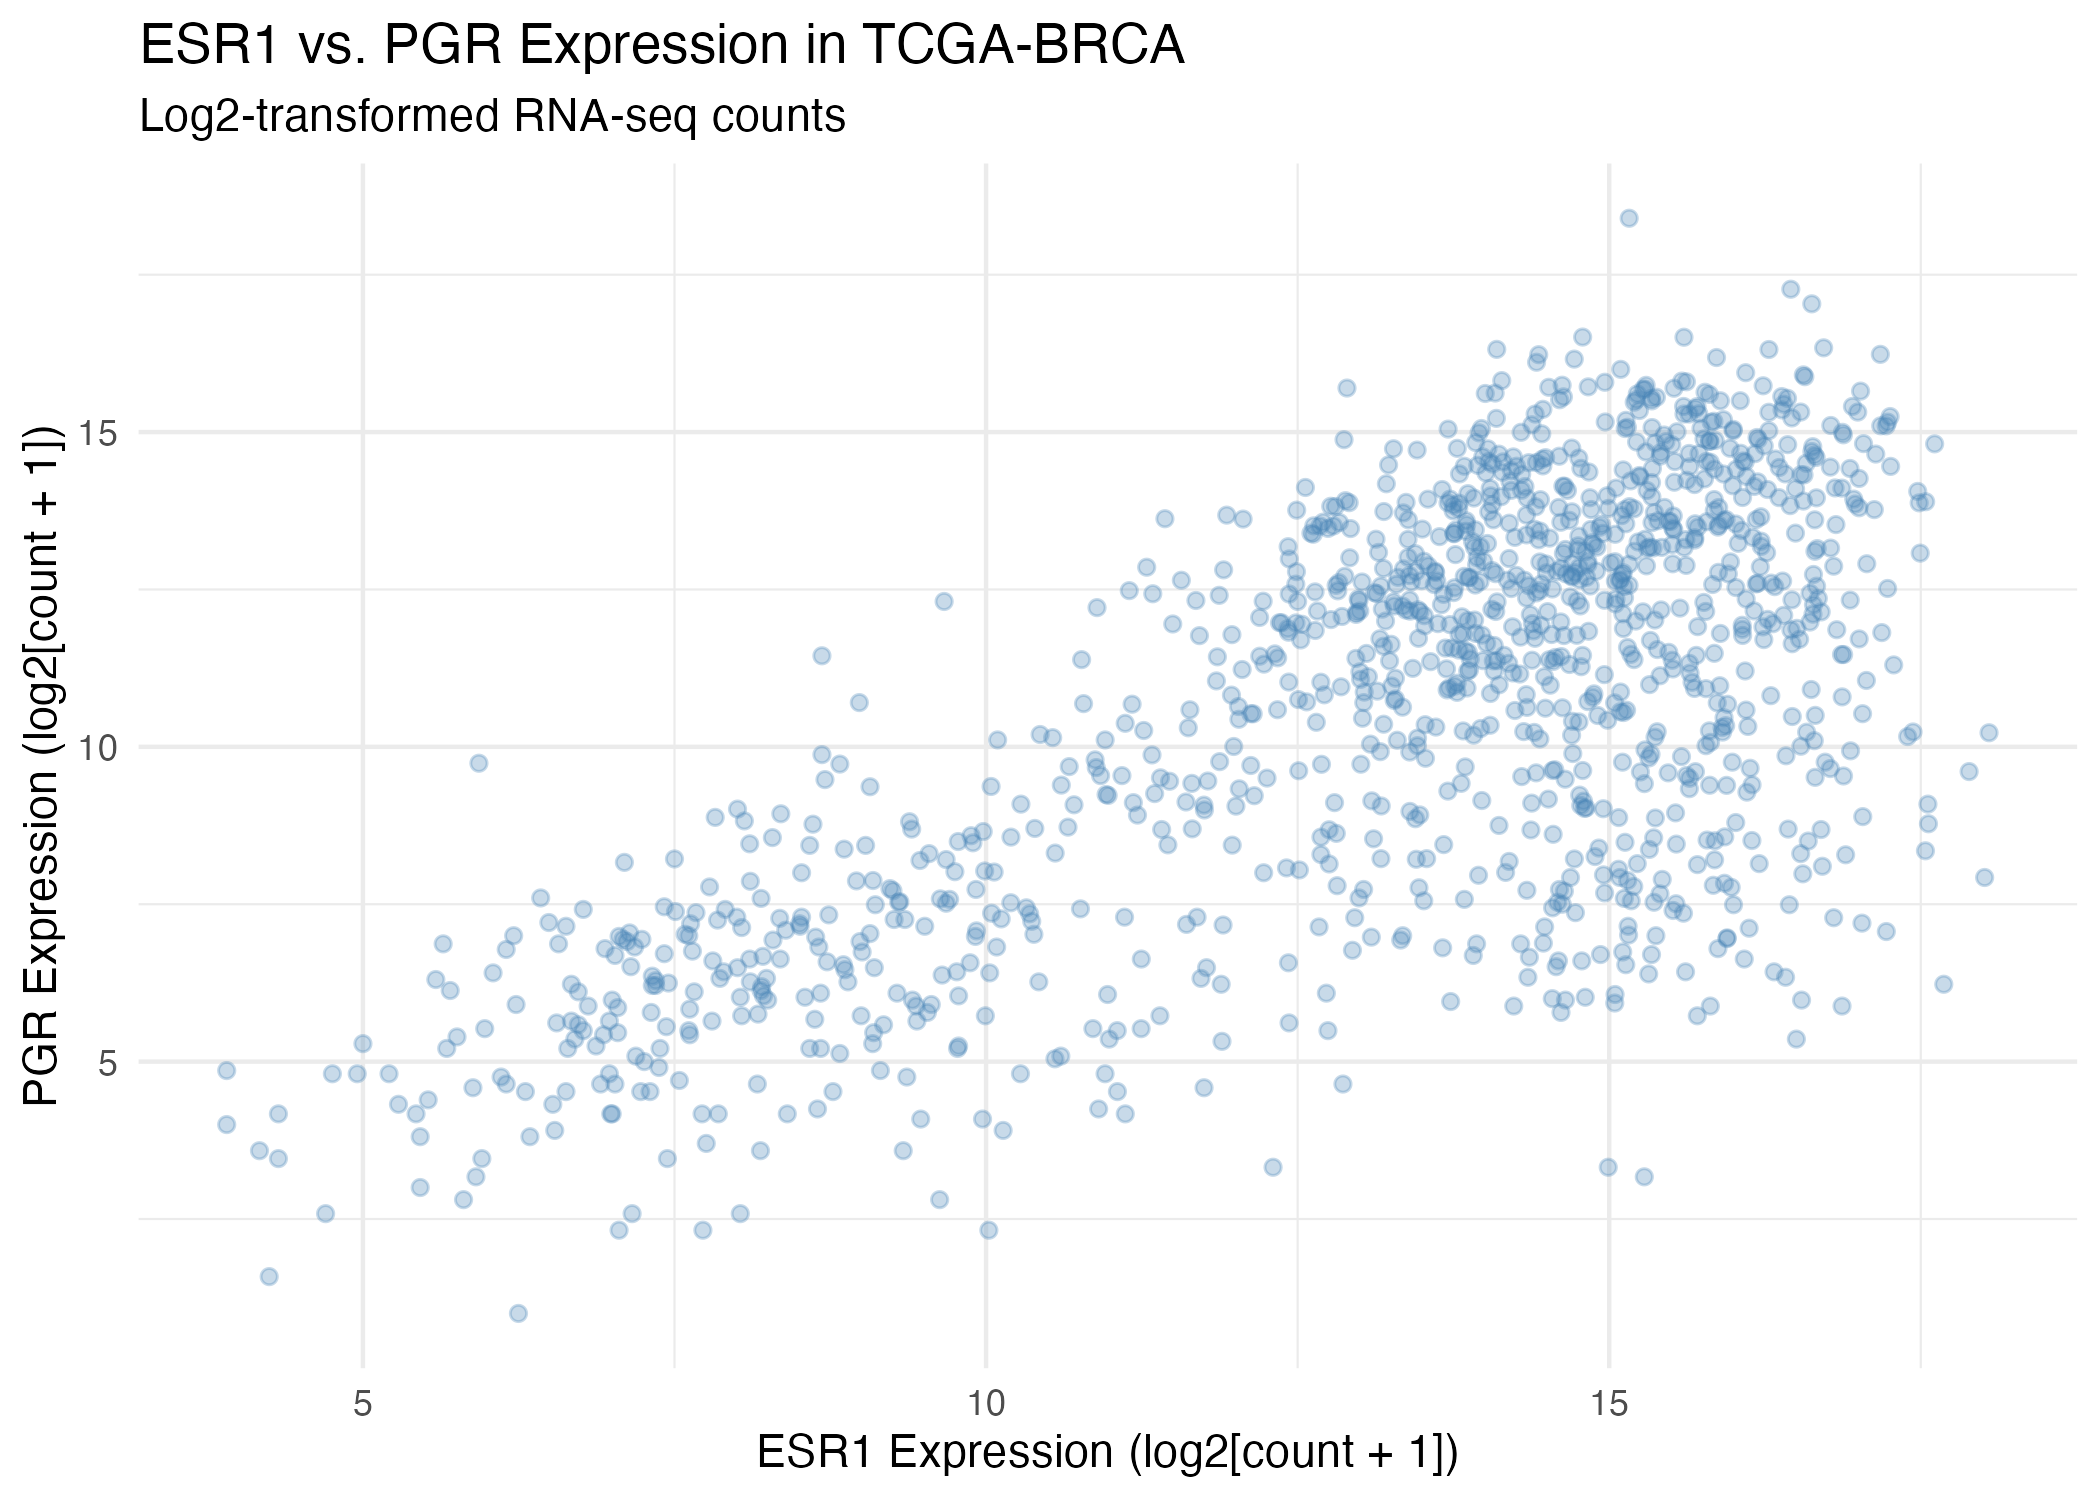
\includegraphics[width=\linewidth,height=0.52\textheight,keepaspectratio]{figures/scatter_plot.png}
\caption{Relationship between log2-transformed \textit{ESR1} and \textit{PGR} RNA-seq counts across TCGA-BRCA samples.}
\label{fig:scatter}
\end{figure}
\subsection{\textit{ESR1} Expression Across Breast Cancer Subtypes}
The box plot (Figure 3) compared log2-transformed \textit{ESR1} counts across PAM50 breast cancer subtypes. Luminal A and Luminal B samples generally exhibited higher \textit{ESR1} expression, while Basal samples showed substantially lower expression. Differences in the spread and distribution of values within each subtype demonstrated variation among individual samples.

\begin{figure}[H]
\centering
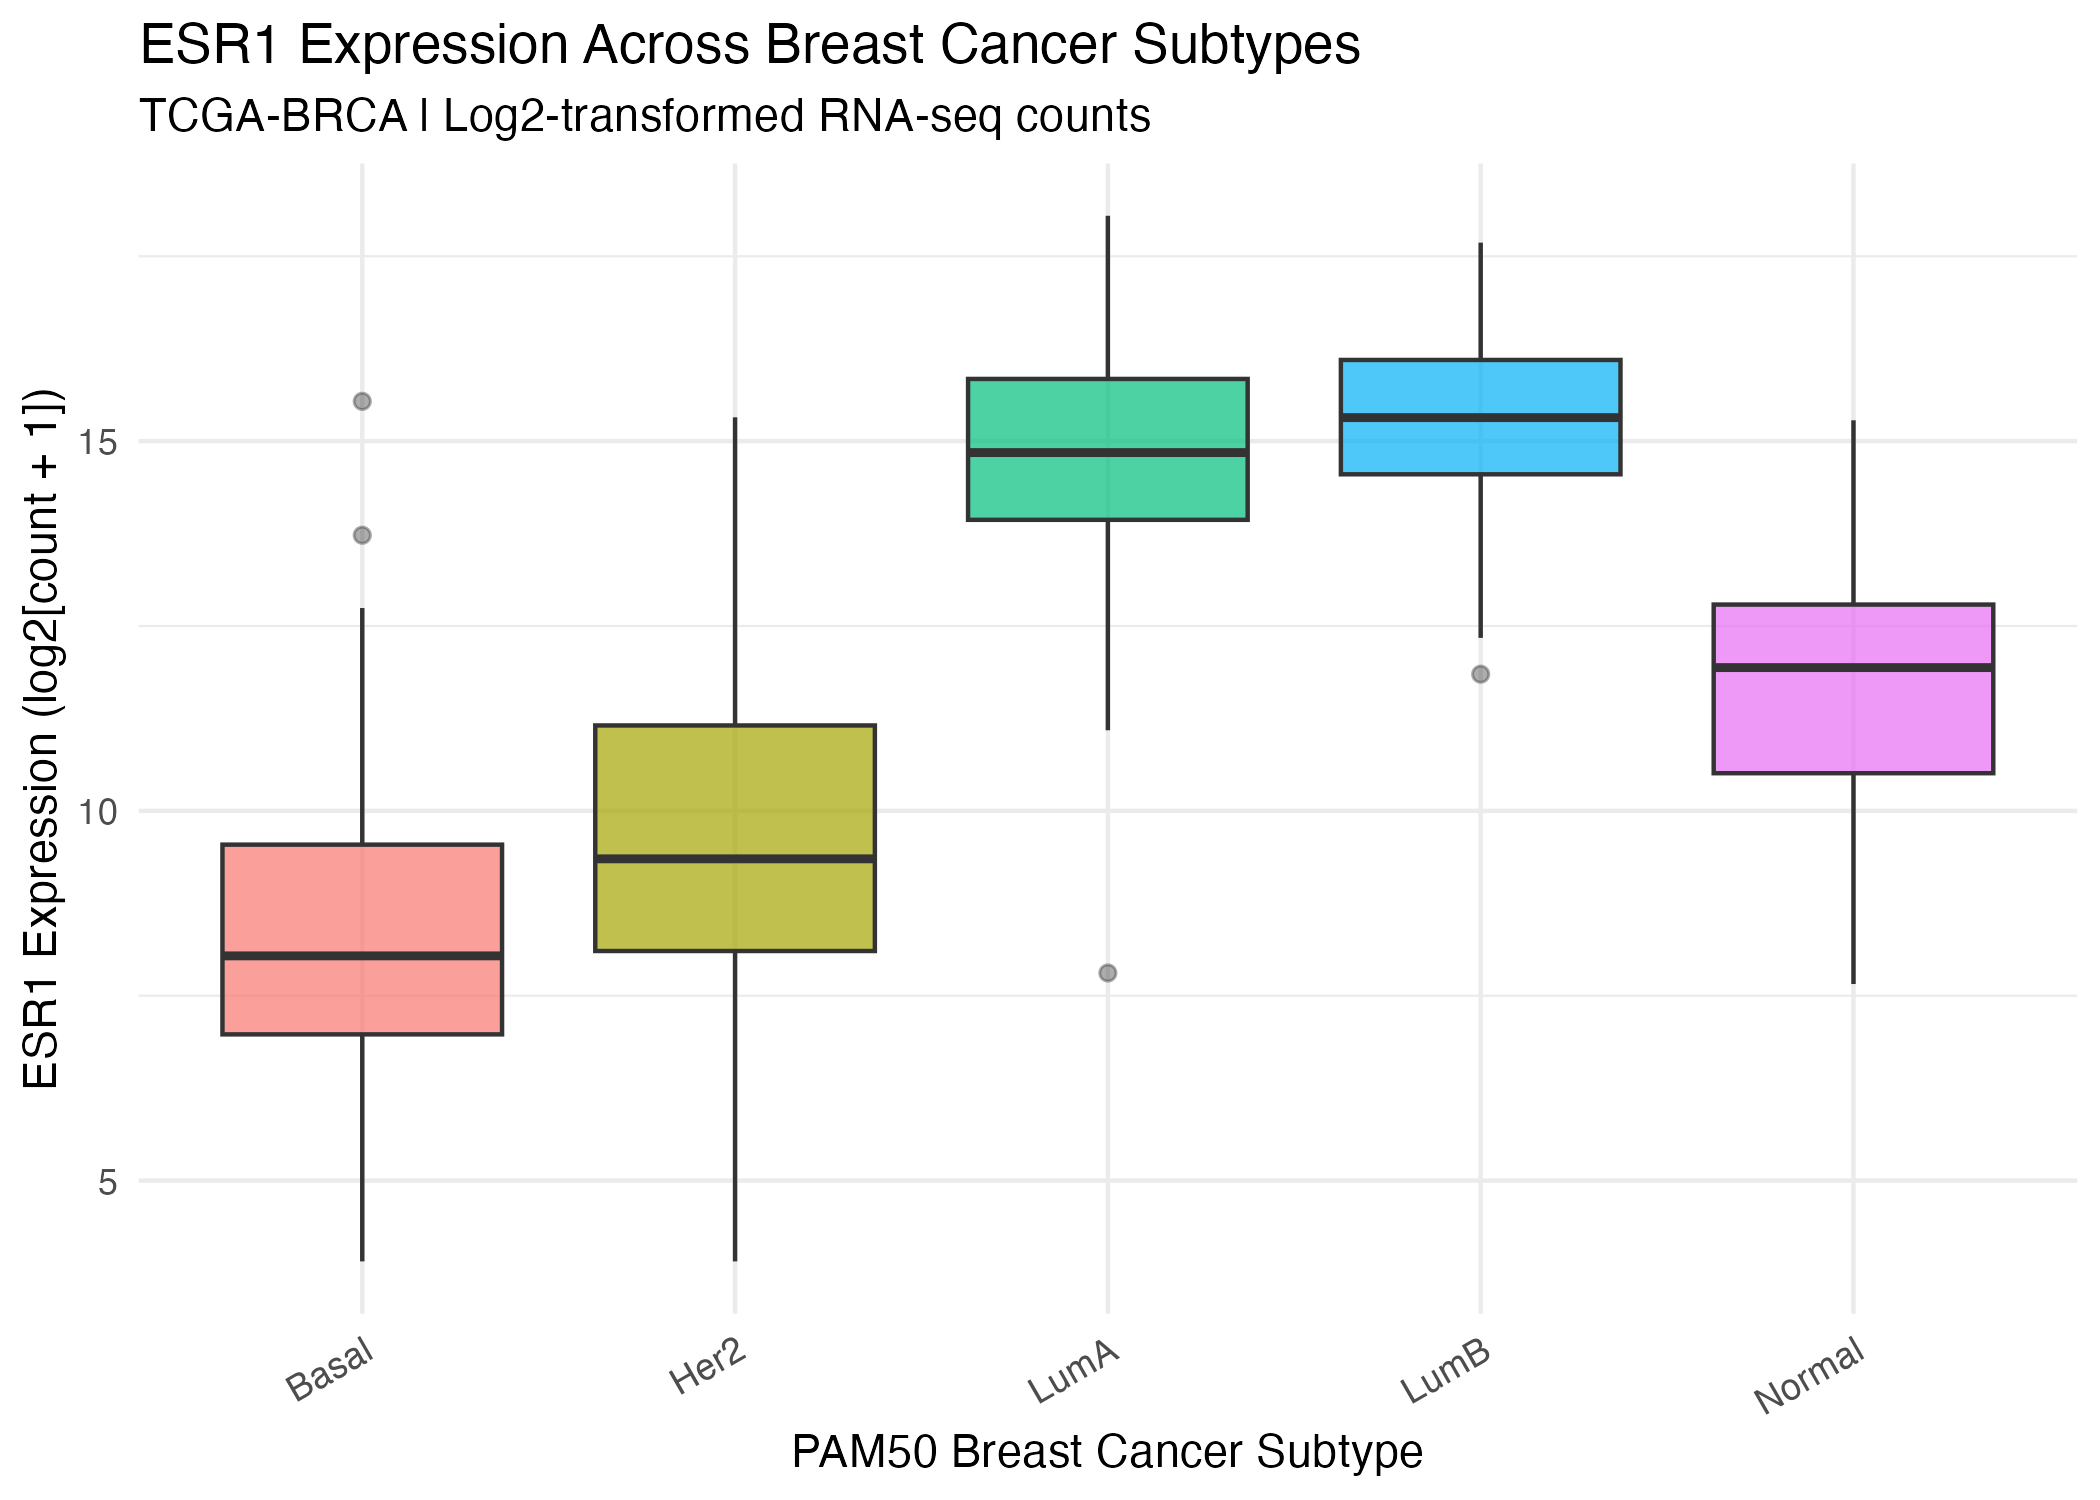
\includegraphics[width=\linewidth,height=0.52\textheight,keepaspectratio]{figures/boxplot.png}
\caption{Box plot comparing log2-transformed \textit{ESR1} RNA-seq counts across PAM50 breast cancer subtypes.}
\label{fig:boxplot}
\end{figure}
\subsection{Heatmap of Gene Expression Patterns}
The heatmap (Figure 4) displayed the 10 genes with the highest average raw RNA-seq counts across the dataset. Following log2 transformation, hierarchical clustering was used to organize genes and samples according to similarities in their expression patterns. The PAM50 subtype annotation provided additional context for comparing gene expression across breast cancer subtypes. Differences in color intensity indicated variation in RNA-seq counts among genes and samples.

\begin{figure}[H]
\centering
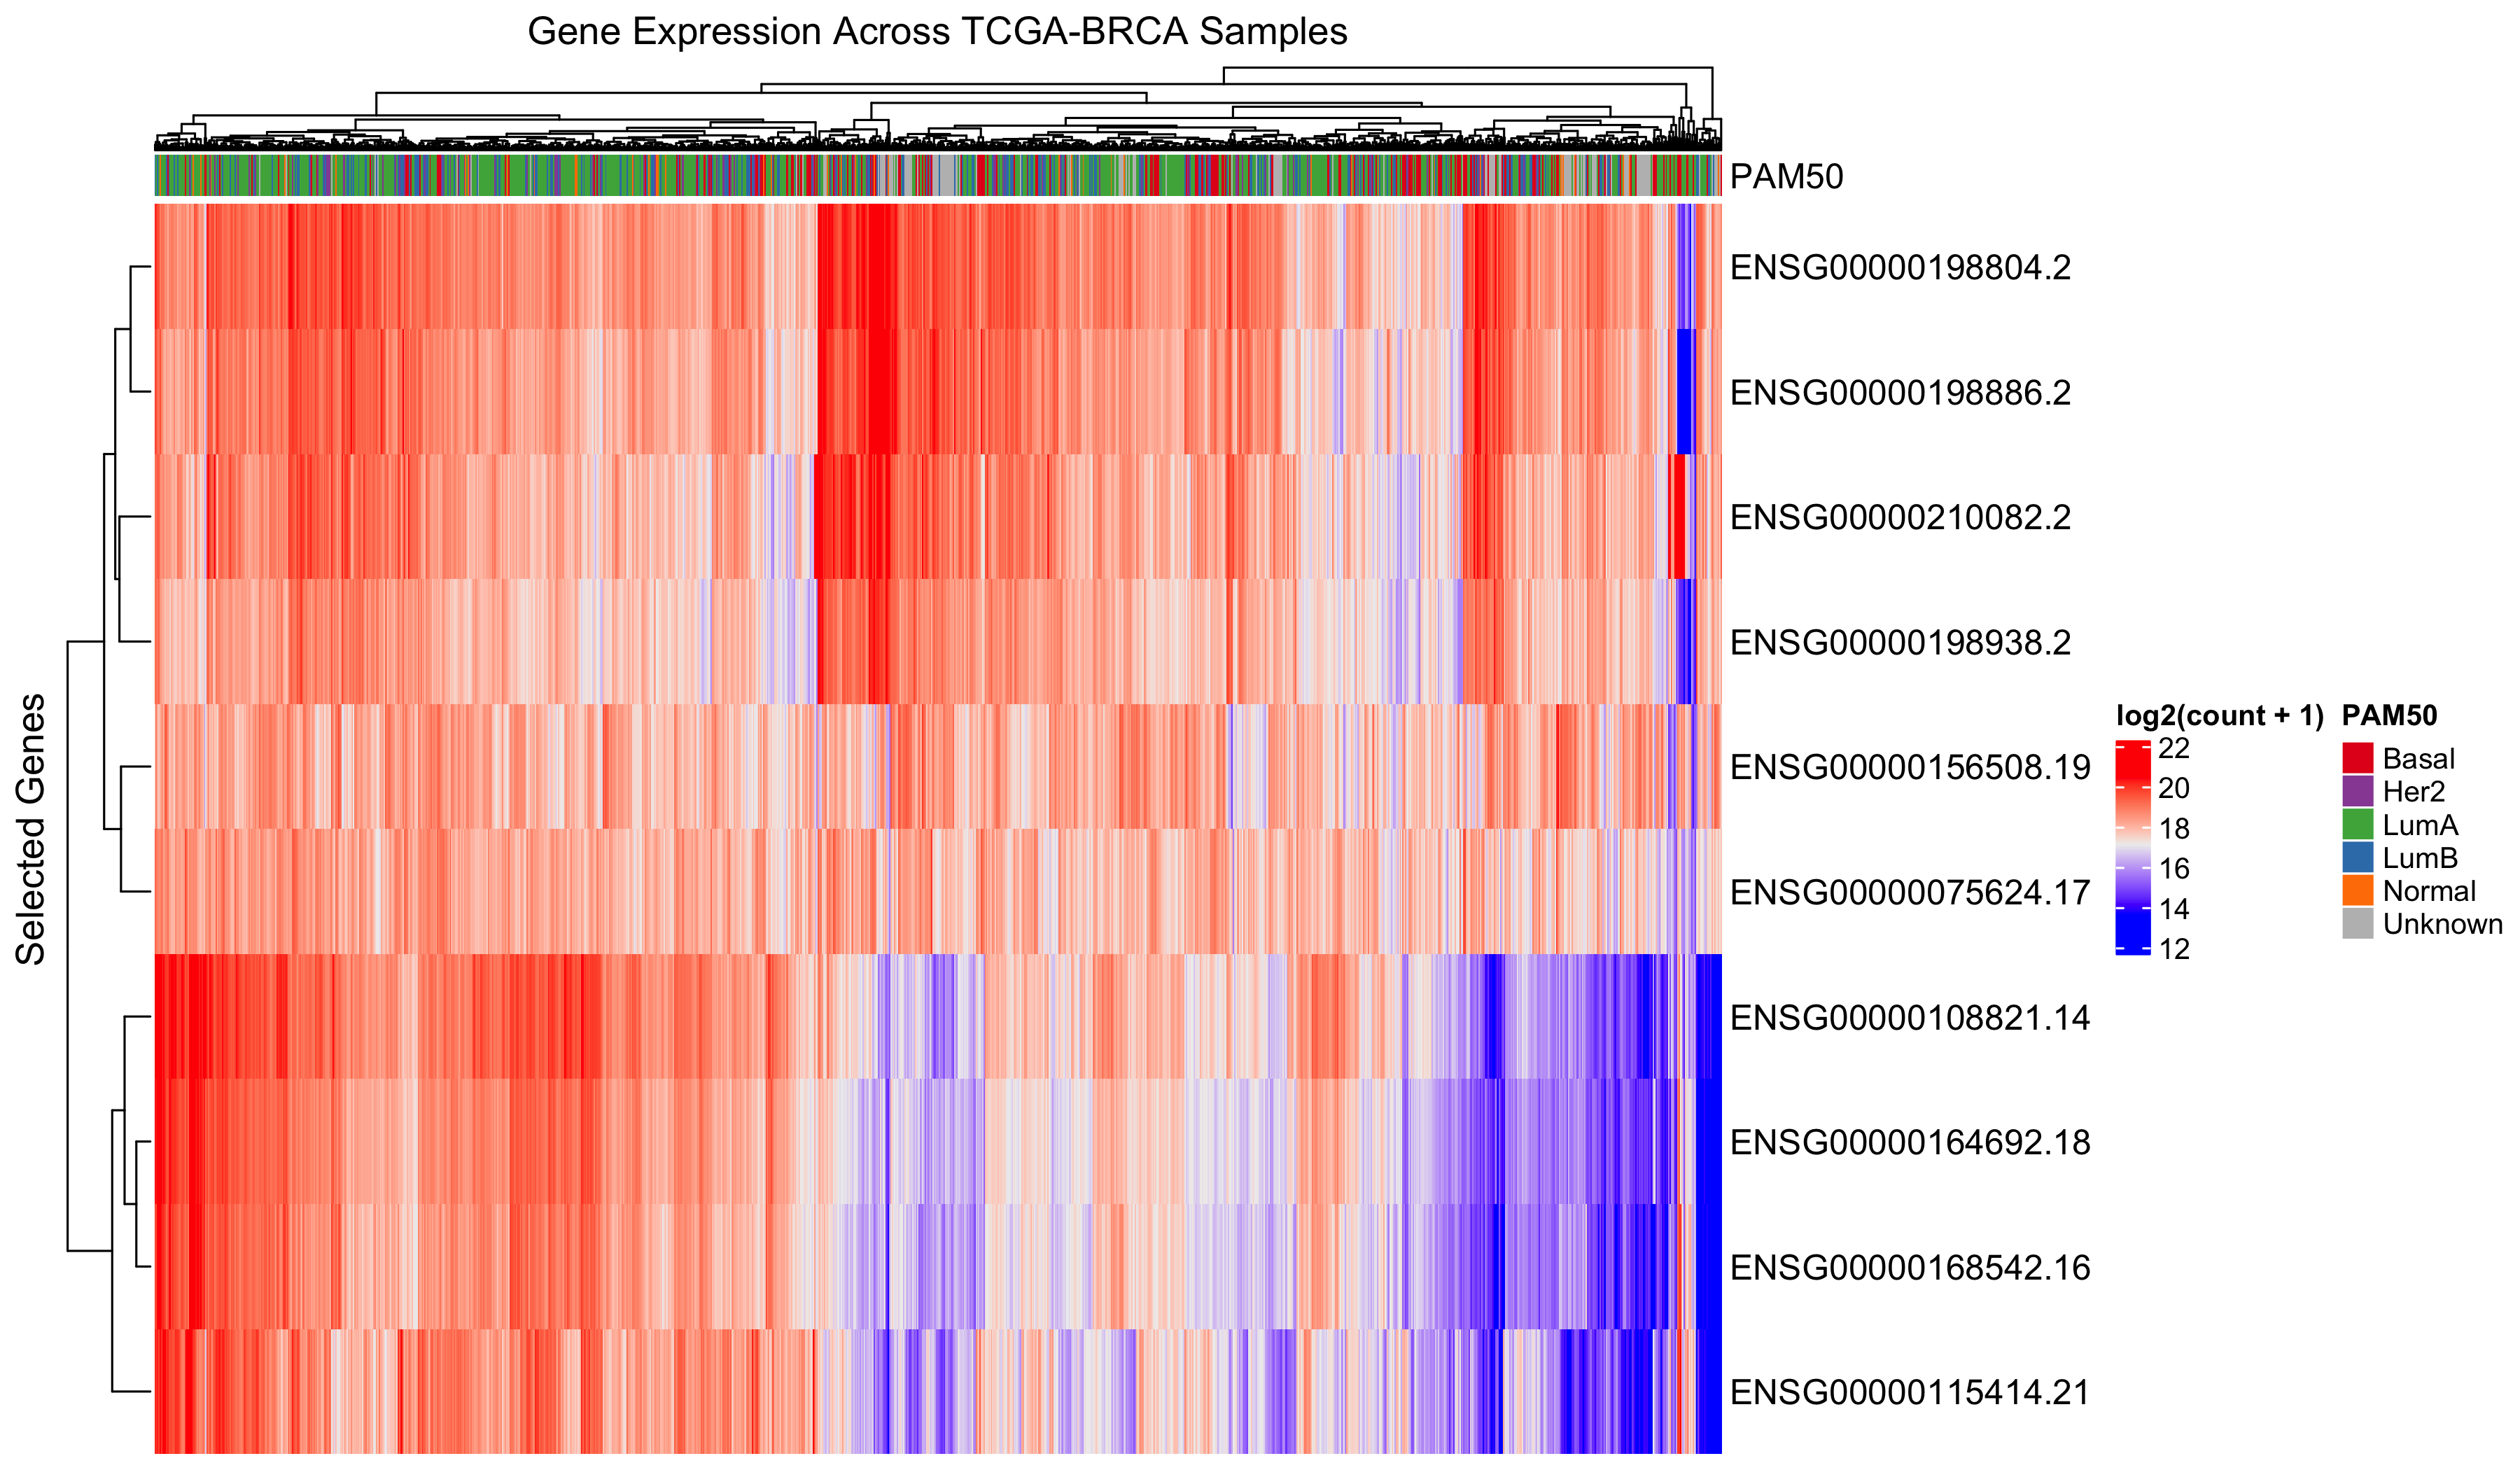
\includegraphics[width=\linewidth,height=0.70\textheight,keepaspectratio]{figures/heatmap.png}
\caption{Heatmap of log2-transformed RNA-seq counts for the 10 genes with the highest average raw counts, with PAM50 subtype annotations.}
\label{fig:heatmap}
\end{figure}
\subsection{Density Plot of \textit{ESR1} Expression}
The density plot (Figure 5) provided an additional comparison of \textit{ESR1} expression distributions across PAM50 subtypes. Luminal A and Luminal B samples were generally concentrated at higher log2-transformed expression values, whereas Basal samples were concentrated at lower values. Overlap among the density curves demonstrated variation both within and between breast cancer subtypes, complementing the differences observed in the box plot.

\begin{figure}[H]
\centering
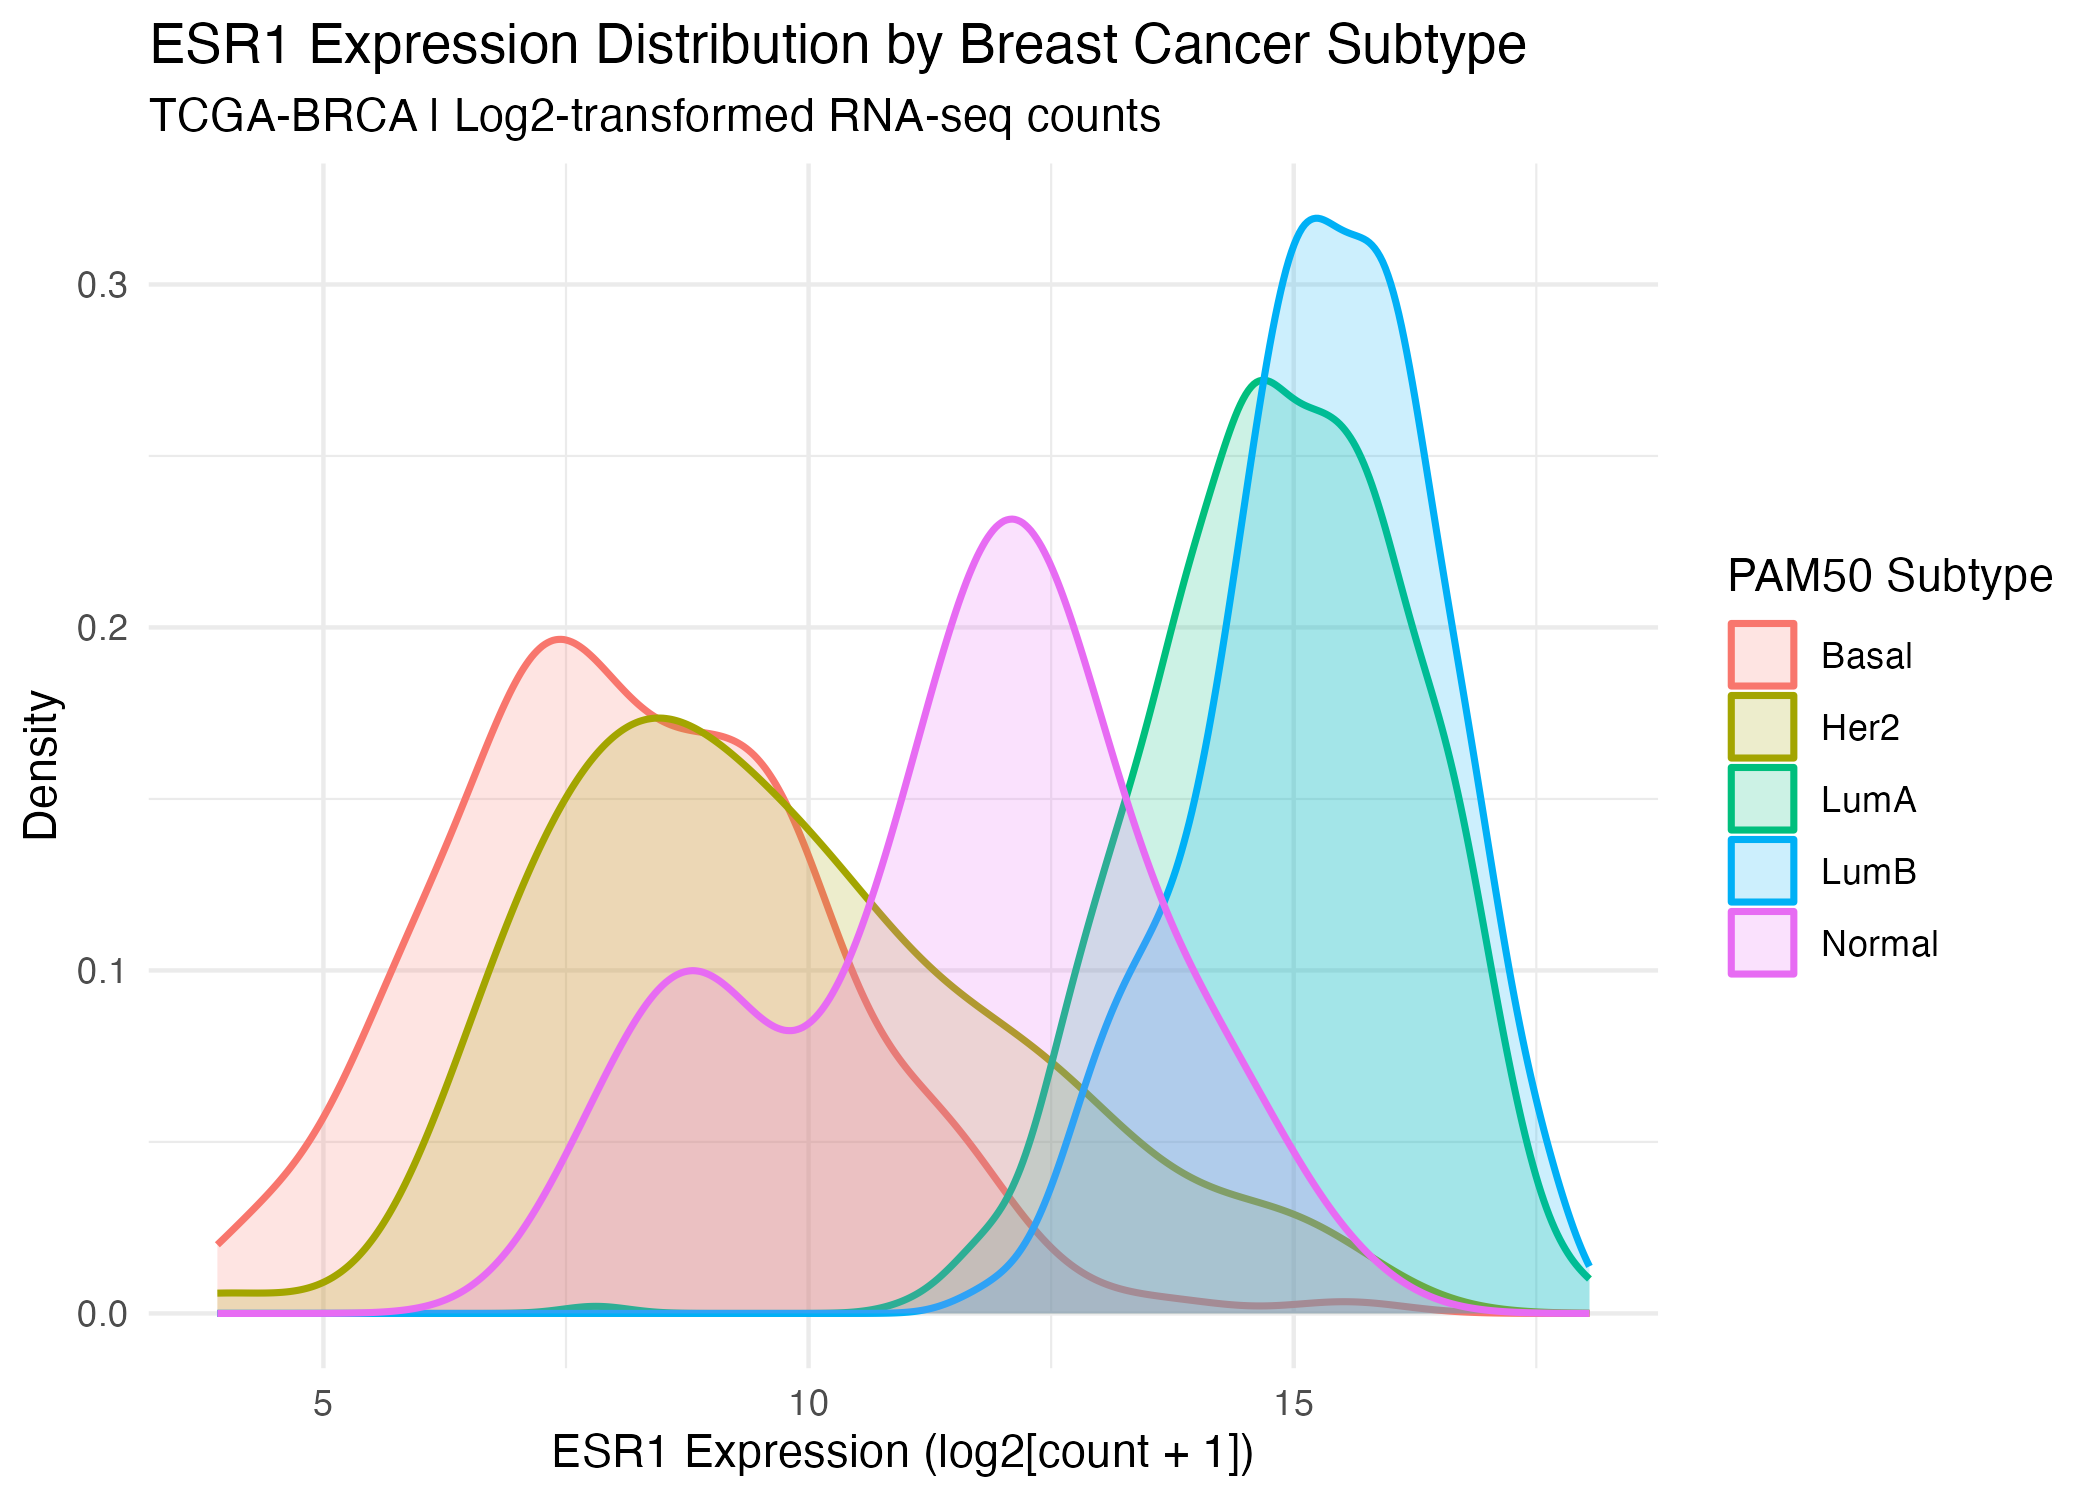
\includegraphics[width=\linewidth,height=0.52\textheight,keepaspectratio]{figures/density_plot.png}
\caption{Density distributions of log2-transformed \textit{ESR1} RNA-seq counts across PAM50 breast cancer subtypes.}
\label{fig:density}
\end{figure}
\subsection{Interpretation and Limitations}
Overall, the results demonstrated substantial variation in \textit{ESR1} and \textit{PGR} RNA-seq counts across TCGA-BRCA samples. The subtype comparisons showed higher \textit{ESR1} counts in Luminal A and Luminal B samples relative to Basal samples, consistent with the biological relevance of estrogen receptor signaling in breast cancer classification.

These findings should be interpreted as descriptive patterns rather than evidence of statistically significant differences. Because the analysis used raw, unnormalized RNA-seq counts, differences in sequencing depth and other technical factors may influence comparisons between samples. Additionally, no inferential statistical tests were conducted, limiting conclusions about the strength or statistical significance of the observed relationships.

\section*{References}
\noindent Cancer Genome Atlas Network. (2012). Comprehensive molecular portraits of human breast tumours. Nature, 490, 61--70. \url{https://doi.org/10.1038/nature11412}\par\vspace{0.7em}
\noindent National Cancer Institute. (n.d.). Genomic Data Commons Data Portal. \url{https://portal.gdc.cancer.gov/}\par\vspace{0.7em}
\noindent Parker, J. S., et al. (2009). Supervised risk predictor of breast cancer based on intrinsic subtypes. Journal of Clinical Oncology, 27(8), 1160--1167. \url{https://doi.org/10.1200/JCO.2008.18.1370}\par\vspace{0.7em}
\end{document}